\begin{quote}
  \textit{L’histoire se fait avec des documents. Les documents sont les traces qu’ont laissées les pensées et les actes des hommes d’autrefois.} [...] \textit{Faute de documents, l’histoire d’immenses périodes du passé de l’humanité est à jamais inconnaissable. Car rien ne supplée aux documents : pas de documents, pas d’histoire.}\footnote{Charles-Victor Langlois et Charles Seignobos, \og La recherche des documents (heuristique) \fg, dans \textit{Introduction aux études historiques}, collection Bibliothèque idéale des sciences sociales, ENS édition, 2014.}
\end{quote}


\lettrine{C}{'est dans} \textit{Introduction aux études historiques} que Charles-Victor Langlois et Charles Seignobos jalonnent une méthode historique scientifique qui se structure en deux temps : l'heuristique et l'herméneutique. La première est une activité partagée avec les métiers des archives et des bibliothèques. Elle désigne l'opération matérielle et laborieuse qui consiste à repérer, localiser et rassembler les sources avant même de pouvoir les interroger.

%reprendre la formulation de l'accroche

Or, ce même terme d'\og heuristique \fg{} connaît, un siècle plus tard, une deuxième vie dans le champ de l'informatique et de l'intelligence artificielle, où il désigne les méthodes de résolution approximative d'un problème~: des règles pragmatiques permettant à une machine de trouver une solution satisfaisante là où un calcul exhaustif et complet serait coûteux. Le domaine de la vision par ordinateur appliquée aux corpus historiques fait alors cohabiter les deux traditions de l'heuristique : celle du chercheur et de la chercheuse qui sélectionne ses sources, et celle, computationnelle, qui intervient au sein même des modèles d'apprentissage profond car ils reposent fondamentalement sur une optimisation statistique. Ces deux définitions convergent aujourd'hui vers de nouveaux modes d'exploration, donnant naissance à une heuristique historique \og augmentée \fg. C'est cette rencontre technologique au cœur des documents, ainsi que les glissements méthodologiques qu'elle induit, qui constitue le point de départ de ce travail.

Les historiens ont rapidement intégré les outils numériques dans leur travail\footnote{Philippe Rygiel, \og L’ordinateur, le réseau et l’écriture de l’histoire. Matériaux pour l’histoire de notre temps \fg, dans \textit{L’historien face à l’ordre informatique : classification et histoire}, n°82, pp.75-79, 2006.} comme en témoigne en France la publication en 1979 par l'\gls{irht} de la revue \textit{Le Médiéviste et l'Ordinateur}. La question de l'image et de son exploitation informatique reste une niche, mais nous notons ici plusieurs articles s'intéressant à la mise en index et en base de données sur le sujet de l'iconographie médiévale au milieu des années 1980, comme ici avec \textit{À la recherche des images : vidéo-disque et iconographie}\footnote{François Garnier, \og À la recherche des images: vidéo-disque et iconographie\fg, dans \textit{Le Médiéviste et l'Ordinateur}, n°12, pp. 7-8, 1984} de François Garnier en 1984 et \textit{Couverture fascicule par et pour la recherche d'images : EXPRIM}\footnote{Marion Crehange, \og Couverture fascicule par et pour la recherche d'images : EXPRIM\fg, dans \textit{Le Médiéviste et l'Ordinateur}, n°19, pp. 15-21, 1988} de Marion Crehange en 1988. 
La question de l’usage de la vision artificielle appliquée aux humanités fait ses premiers pas dans les années 1990 avec le développement de l’analyse automatique de documents (\gls{diar}) et du traitement de texte. Ce domaine utilise l’apprentissage machine (machine learning) pour analyser et reconnaître des images, vidéos ou objets 3D. Cette discipline de l’informatique permet à un programme d’apprendre à partir de données existantes pour traiter ensuite de nouvelles informations. Les recherches se focalisent alors sur la reconnaissance de caractères imprimés (\gls{ocr}) et manuscrits (\gls{htr}), avec des applications concrètes dans l’automatisation postale. Aux frontières du monde des ingénieur\pmm e\pmm s et des historien\pmm ne\pmm s, des conférences liées à l’étude des documents par des méthodes de vision par ordinateur comme l’\gls{icfhr} et l’\gls{icdar} vont apparaître et structurer la recherche interdisciplinaire sous un format de conférences et de compétitions régulières.

En 1997, le lancement de Gallica par la \gls{bnf} marque un tournant dans la mise à disposition numérique des sources en France et le début de la transhumance informatique du patrimoine littéraire et artistique avec Google Books en 2004 ou Europeana en 2008. Si la discipline historique a réussi à apprivoiser l’informatique — principalement par le biais de la bureautique, de la mise en placede moteurs de recherche institutionnels\footnote{Caroline Muller et Frédéric Clavert, \og D’étranges territoires de l’histoire : les moteurs de recherche et interfaces de découverte \fg, dans \textit{Écrire l’histoire, Gestes et expériences à l’ère numérique}, éditions Armand Colin, 2025.}; enfin, la numérisation des collections des archives et des bibliothèques patrimoniales\footnote{Deanna Marcum et Roger C. Schonfeld, \og Implications \fg, dans \textit{Along Came Google : A History of Library Digitization}, éditions Princeton University Press, 2023} — l’efficacité des méthodes utilisant des technologies de \textit{machine learning} ouvre la possibilité du traitement automatique de grandes masses documentaires, et stimule donc le besoin de méthodes d’heuristique historique adaptées à cette nouvelle ère.

Si la période des années 1990-2000 était celle des précurseurs, l’apparition durant la décennie 2010 de l’apprentissage profond (\textit{deep learning}) et de son tournant visuel fait entrer la discipline dans une ère de maturité\footnote{Alex Krizhevsky, Ilya Sutskever, Geoffrey E. Hinton, \og ImageNet Classification with Deep Convolutional Neural Networks \fg, dans \textit{Communications of the ACM}, N°60, vol 6, 2012.}. La question n’est plus si ces technologies peuvent être utilisées pour l’heuristique historique, mais comment les utiliser le plus efficacement, et jusqu’où peuvent-elles être poussées. À titre d'exemple, il s'est publié autant de jeux de données historiques pour l’entraînement de modèles durant la seule année 2017 qu’entre 2009 et 2014\footnote{Konstantina Nikolaidou, \og A survey of historical document image datasets \fg, dans \gls{ijdar}, n°25, vol 4, pp. 305-338, 2022.}. En 2018, l’\gls{ephe} rend publique la première version d’eScriptorium\footnote{B. Kiessling, R. Tissot, P. Stokes and D. Stökl Ben Ezra, \og eScriptorium : An Open Source Platform for Historical Document Analysis \fg, durant 2019 \gls{icdarw}, Sydney, NSW, Australia, 2019, pp. 19-19, doi : 10.1109/ICDARW.2019.10032}, une plateforme de mise à disposition aux chercheurs de technologies de segmentation et de reconnaissance du texte manuscrit (\gls{htr}), et en 2019 la \gls{bnf} rend public son outil d’indexation automatique d’images et de recherche nommé GallicaPix\footnote{Marion Charpier, \textit{Computer Vision appliquée à l’analyse de sources visuelles médiévales : exploration et implications historiques}, 2023}. En 2020, Tom Monnier et Mathieu Aubry publient \textit{DocExtractor}\footnote{Tom Monnier, Mathieu Aubry, \og docExtractor : An off-the-shelf historical document element extraction \fg,dans \textit{2020 17th International Conference on Frontiers in Handwriting Recognition} (\gls{icfhr}), pp. 91-96, 2020, DOI : 10.1109/ICFHR2020.2020.00027}, un démonstrateur de segmentation automatique en utilisant des données synthétiques. Ces initiatives illustrent la transition vers une étape charnière pour les sciences historiques : celle du déploiement d’outils et d’environnements de travail clés en main, démocratisant l’accès aux méthodes de vision par ordinateur\footnote{Francesco Lombardi, Simone Marinai, \og Deep Learning for Historical Document Analysis and Recognition—A Survey \fg, dans \textit{Journal of Imaging}, n°6, vol 10, pp. 110-140, 2020, DOI :10.3390/jimaging61001104} et réfléchissant aux impacts de la technique sur la discipline historique.


Aujourd'hui, l'intégration de la vision artificielle dans les sciences historiques se divise principalement en deux catégories.
\begin{itemize}
    \item L'automatisation de la transcription du texte, nommée \textit{Optical Character Recognition} (\gls{ocr}) pour les caractères imprimés, \textit{Handwritten Text Recognition} (\gls{htr}) pour les écritures manuscrites, mais également la segmentation à la ligne ou la reconnaissance d'écritures.
    \item Le travail sur la détection et la segmentation de parties du document : on peut alors essayer de segmenter toute la mise en page du document avec l'\gls{olr}, ou plus simplement détecter automatiquement la présence de certains attributs.
\end{itemize}

C'est dans ce deuxième champ d'application que s'inscrit le développement de l'application AIKON par le laboratoire IMAGINE au sein du \gls{ligm}. L'élaboration de cet outil s'insère dans plusieurs programmes de recherche consacrés à la vision artificielle appliquée aux sciences historiques, à l'image des projets ANR \gls{vhs}\footnote{Coordonné par Alexandre Guilbaud, \gls{vhs} : \textit{Computer vision and Historical Analysis of Scientific Illustration Circulation}, Sorbonne Université et ENPC, URL :  \href{https://vhs.hypotheses.org/}{https://vhs.hypotheses.org/}} et \gls{eida}\footnote{Coordonné par Matthieu Husson, \gls{eida} : \textit{Éditer et analyser les diagrammes astronomiques historiques avec l’intelligence artificielle},  Observatoire de Paris \& ENPC, URL : \href{https://eida.hypotheses.org/}{https://eida.hypotheses.org/}}.
AIKON ambitionne de proposer un environnement qui \og accompagne les utilisateurs tout au long du processus, de la constitution du corpus au traitement algorithmique et à la validation des résultats, sans nécessiter de compétences techniques particulières \fg\footnote{S. Albouy, S. Norindr, P. Kervegan, F. Aouinti, C. Grometto, R. Champenois, A. Guilbaud, M. Husson, S. Lazaris, M. Aubry, \textit{AIKON: A Modular Computer Vision Platform for Historical Corpora}, 2025, URL :  \href{https://hal.science/hal-05248250}{https://hal.science/hal-05248250}}. Concrètement, la plateforme permet aux historiens d'importer rapidement des corpus numérisés via un manifeste \gls{iiif}, de détecter et de corriger la segmentation des illustrations, d'identifier des motifs similaires à travers différentes sources, de vectoriser des diagrammes scientifiques, et de regrouper visuellement les éléments pertinents pour enrichir l'heuristique des documents manuscrits et imprimés pour les historiens des sciences.

\begin{figure}[h]
	\centering
	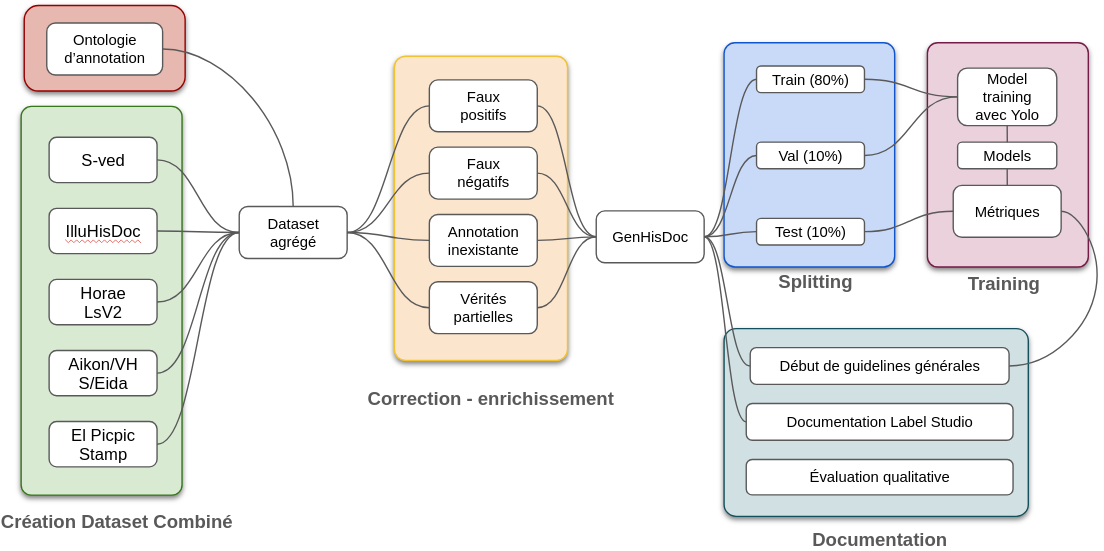
\includegraphics[scale=0.5]{img/GenHisDocOrganisation.png}
	\caption{Organisation du projet de stage et structuration des corpus dans GenHisDoc}
	\label{fig:GenHisDoc}
\end{figure}


C'est dans ce contexte qu'a eu lieu, entre début mai et fin juillet 2026, le stage au sein de l'équipe en charge du développement d'AIKON dans le laboratoire IMAGINE à l'\gls{enpc}. L'objectif principal était de construire un corpus d'entraînement de modèles de détection pour la plateforme. Pour arriver à cette fin, le travail a nécessité la définition d'une méthodologie préalable de constitution d'un corpus et de l'élaboration d'un vocabulaire d'annotation contrôlé en collaboration avec les projets \gls{vhs} et \gls{eida},  puis la construction d'un \textit{pipeline} d'entraînement d'un modèle de détection et de ses métriques pour l'évaluer. Plutôt que de constituer un jeu de données en partant de zéro, nous nous sommes intéressés à la question de la réutilisation et de la combinaison de travaux similaires dont les droits nous le permettaient. En plus de cette question de la réutilisation des matériaux de la recherche, nous nous sommes également intéressé à la capitalisation sur les matériaux d'annotation déjà produits par les utilisateurs d'AIKON. Réutiliser des données déjà annotées ajoute une couche de complexité à la constitution d'un jeu de données et nous avons exploré certaines stratégies de contournement, notamment pour les éléments comme les estampilles, pour diminuer l'effort d'annotation d'un élément relativement ignoré des jeux de données à visée patrimoniale.


Ce travail soulève une question : comment tous ces choix, qui impliquent une mise en données, conditionnent-t-ils l'efficacité de la vision par ordinateur dans le domaine de l'heuristique, c'est-à-dire la capacité à travailler sur un document historique et à en produire une analyse pertinente et scientifique ?

Dans un premier temps, nous dresserons un état de l'art de la rencontre entre vision par ordinateur et recherche historique. Nous retracerons d'abord l'évolution des technologies d'analyse d'images documentaires, depuis l'origine de la vision artificielle jusqu'à l'avènement des modèles vision-langage et des approches \textit{zero-shot}, en passant par les architectures \gls{yolo} et \gls{detr}. Nous analyserons ensuite la manière dont la communauté des historiennes et des historiens s'approprie ces outils, en observant les transformations de la pratique scientifique, la fabrique de la vérité de terrain et l'émergence d'une « nouvelle économie de l'érudition ». Enfin, nous situerons ce travail au sein de l'écosystème de la recherche en présentant le projet Aikon, ses objectifs scientifiques et ses réalisations techniques, tout en le confrontant aux autres initiatives nationales et internationales de vision artificielle historique.

Ensuite, nous détaillerons le processus de construction d'un corpus de numérisations adapté aux exigences de la vision artificielle. Nous traiterons d'abord des enjeux de la préparation d'une campagne d'annotation, qui nécessite de formaliser une ontologie appliquée aux documents historiques, de tracer des frontières sémantiques claires face aux cas limites et de rédiger des consignes rigoureuses. Nous expliciterons ensuite la constitution concrète du corpus, en abordant la réutilisation de jeux de données existants (tels que S-VED, IlluHisDoc ou Horae) et la récupération des métadonnées d'Aikon via \gls{iiif}, ainsi que les défis techniques liés à l'harmonisation des formats et à la correction des annotations sous Label Studio.

Enfin, nous analyserons l'entraînement et l'évaluation du modèle entraîné sur notre jeu de données. Après avoir détaillé le rôle et l'impact des hyperparamètres sur la dynamique d'apprentissage, nous présenterons la méthodologie d'évaluation mise en œuvre et analyserons les résultats obtenus sur la détection des différentes catégories d'objets (illustrations, ornements, lettrines, tampons et tables). Pour finir, nous confronterons ces métriques aux limites observées afin de dégager des pistes d'amélioration ciblées, qu'il s'agisse de l'ajustement des paramètres, du perfectionnement du protocole d'évaluation, du raffinage des annotations ou d'une refonte de l'ontologie.














